\section{Solution Design}

This section will describe the solution in terms of the distributed and
concurrent parts of the system and the communication protocols that we have
designed:

\begin{itemize}
\item \textbf{Distribution -- System Architecture}:
  broad view of the system architecture
\item \textbf{Communication Protocols}:
  description of communication protocols. In this section we will expose the
  reason why certain protocols have been chosen and which properties they are
  able to guaranteed for the communication of the system
\item \textbf{Distribution -- Middleware Layer}:
  description of the middleware components and their properties. In this
  section we will explain the design choices in relation to the architectural
  properties that have been chosen for the distributed part of the system
\item \textbf{Concurrency -- Application Layer}:
  description of the application components and their properties. In this
  section we will describe why our design choices leads to a correct concurrent
  system
\item \textbf{Artificial Intelligence (AI)}:
  description of how we solved the problem of computing each agent's path
  in a distributed, multi-agent, dynamic environment.
\end{itemize}


% Distribution - System Architecture
\subsection{Distribution -- System architecture}
As we previously said, our system is a simulator whose computation spreads
across multiple nodes.

We thought it was reasonable to divide our system in four subsystems, in order
to reason more easily about it. An overall view of our architecture is depicted
in Figure \ref{fig:sd-sys-arch-overall}:

\begin{figure}[H]
  \centering
  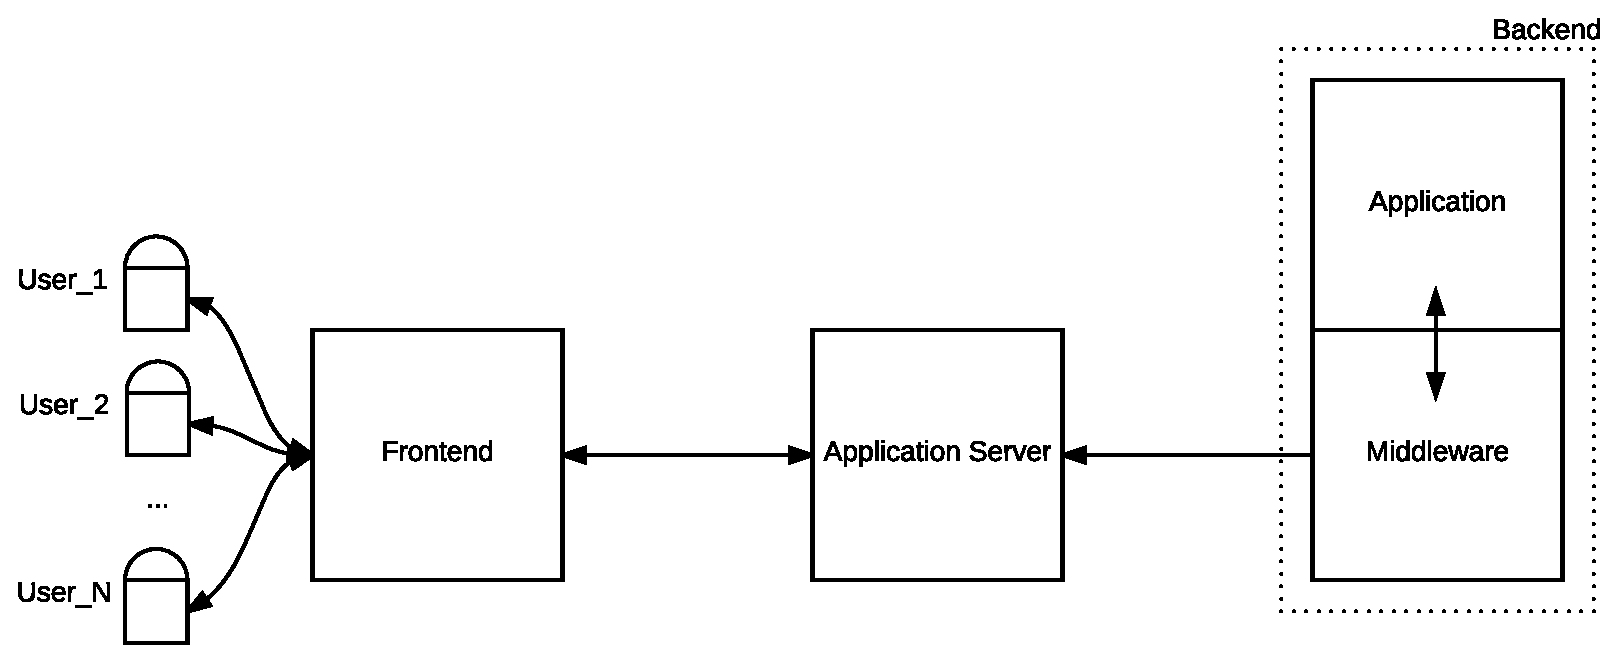
\includegraphics[scale=0.5,keepaspectratio]
    {images/solution/overall-arch.eps}
  \caption{Overall system architecture}
  \label{fig:sd-sys-arch-overall}
\end{figure}

As we can see from Figure \ref{fig:sd-sys-arch-overall}, we have:

\begin{itemize}
  \item a \textbf{Backend}, composed by the \textbf{Application} and the
    \textbf{Middleware} layers;
  \item the \textbf{Application Server}, which is responsible of handling
    information that arrives from the backend and to serve it to the frontend;
  \item a \textbf{Frontend}, which offers streaming services to end users.
\end{itemize}


% Communication Protocols subsection
\subsection{Application}
The Application is composed of two different sub-components (Figure
\ref{fig:sd-app-init}):

\begin{itemize}
  \item \textbf{Application Logic Layer}: handles the application logic
    (slightly abusing the notation, we will often refer to it simply as
    \textit{Application Layer});
  \item \textbf{Interface Layer}: provides the remote services to Application
    Layer by acting as an interface towards the underlying backend layer (i.e.,
    middleware).
\end{itemize}

Thus, the Application Layer communicates with
other applications transparently without knowing if they are local or remote.
This approach has been inspired by the TCP/IP and OSI models.

The following sub-layers compose Interface Layer:

\begin{itemize}
	\item \textit{Session Layer} -
	handles remote connections though a TCP socket;
	\item \textit{Presentation Layer} -
	handles messages formats and conversions;
	\item \textit{Service Layer} -
	implements an event loop with a worker pool and different kind of queues
	for the requests (i.e. synchronous and asynchronous). It converts the
	requests into procedure calls by leveraging a skeleton object.
	Also, it offers the specular service through a stub object and a pipeline,
	necessary to build specific remote requests.
\end{itemize}
\subsubsubsection{Bootstrap}
In order to neatly start the application layer, we have to consider the
dependencies among the entity types exposed in \ref{fig:sd-entity-types-deps}.
Moreover we have to take into account that this layer can not decide by itself
when it is time to start, because this is ruled by the middleware.
The bootstrap process, which mimics the UNIX init (i.e. initd and runlevels)
is divided in two ordered parts:
\begin{enumerate}
	\item \textit{init} - initialize all the sub-layers of each macro layer
	following a bottom up approach (from \verb|interface_layer.session| to \verb|application.scheduling|). The order is inferred by the fact that the upper
	layers need the services provided by the underlying layers to work
	correctly. This event is automatically triggered when the node is created.
	\item \textit{start} - the first tick forwarded from the middleware to the
	application layer through the interface\_layer. As stated, this event is
	exclusively triggered by the middleware.
\end{enumerate}
Also, the application node is divided in two macro layers:
\begin{itemize}
	\item \textit{Interface layer} - provides network services to
	application layer (e.g. session, marshalling, etc.) and acts as an interface
	for the application towards the underlying layers (i.e. middleware);
	\item \textit{Application layer} - implements the city logic
	(e.g. movements of entities in the streets).
\end{itemize}
Each application node contains the \textit{Init} process,
which is the parent of all the application processes.
Init instantiates the resources of each layer triggering the switch of the
interface\_layer state from \verb|inactive| to \verb|ready|.
Also, each sub-layer of interface\_layer has its own pool of LWP.
The application layer initialization completes in the following order:
\begin{enumerate}
	\item \textit{Active} - the entities which moves in the city (e.g. pedestrians);
	\item \textit{Reactive} - the infrastructure of the city (e.g. district);
	\item \textit{Scheduling} - the sub-layer which handles the execution order and
	synchronization signals of each event of the application layer.
\end{enumerate}
Note that the \textit{Passive} entities have no particular dependency. Since
they are stateless and they logically belong to \textit{reactive} entities
(e.g. road signs belong to roads), they will be instantiated along with them.
When the scheduling sub-layer completes its initialization, init signals
the application layer completion to each sub-layer of interface\_layer in the
following order:
\begin{enumerate}
	\item \textit{service} - provides activators and pipelines services to
	application layer;
	\item \textit{presentation} - provides data conversion services;
	\item \textit{session} - provides network connection services
	(e.g. sender, receiver).
\end{enumerate}
This signal triggers the switch of each sub-layer of interface\_layer state from
\verb|ready| to \verb|active|.
The activation order is extremely important to
proactively avoid the lost of messages between remote nodes. Indeed, at this
stage, the application layer is not able to generate or receive messages
because the start message has not been sent by the middleware.
The service and
the presentation layer are activated before the session layer; the latter
exposes a remote communication channel (a connection to a TCP socket).
Moreover, the interface layer follows the nginx concurrency model using a
pool of workers and an event loop to handle multiple concurrent requests
with different queues for different requests (e.g. blocking and asynchronous).
Finally, the application is ready to communicate because each of its layers
has been activated.
% TODO: Review this things

\begin{figure}[H]
  \centering
  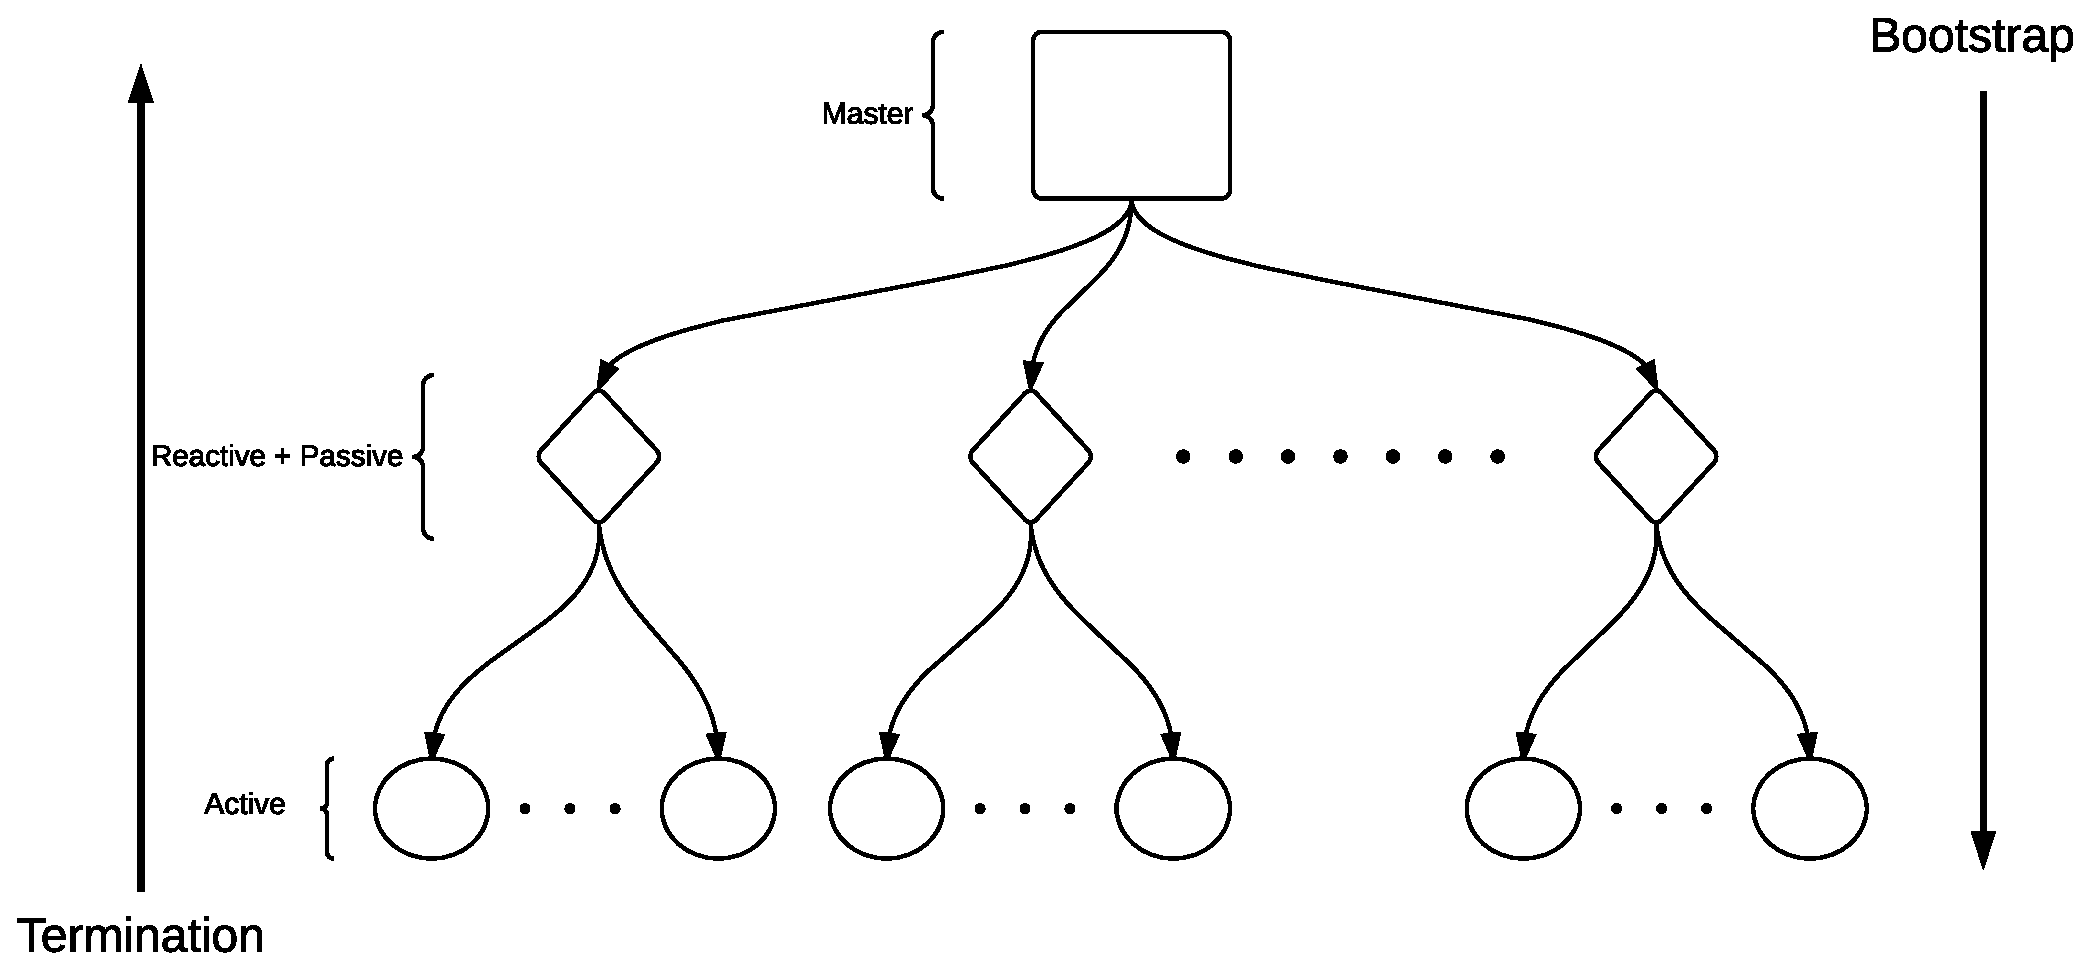
\includegraphics[width=\columnwidth]{images/solution/app_proc_tree.eps}
  \caption{Application process tree}
  \label{fig:app-proc-tree}
\end{figure}

At the end of the bootstrap, the \textit{Init} process has to notify the
middleware layer of the successful completion and the middleware has forwarded
the start message to the application. A crash of the
\textit{Init} process, occurring before the end of the bootstrap,
is signaled to the middleware layer, by the expiration of a timeout from the
middleware side.
Note that this model works also for a bootstrap which is executed starting
from a snapshot of the system, with the only difference consisting in divergent
values of the configuration file. Indeed, we have to use a set of
configurations, which is going to be different for each city.
\subsubsection{Termination}

When describing the shutdown of the whole system, we assumed the application
terminates gracefully.
In this section we show the algorithm we designed to achieve this goal.

As we can see from figure \ref{fig:termination-app}, the termination follows the
opposite order of the bootstrap.

\begin{figure}[H]
  \centering
  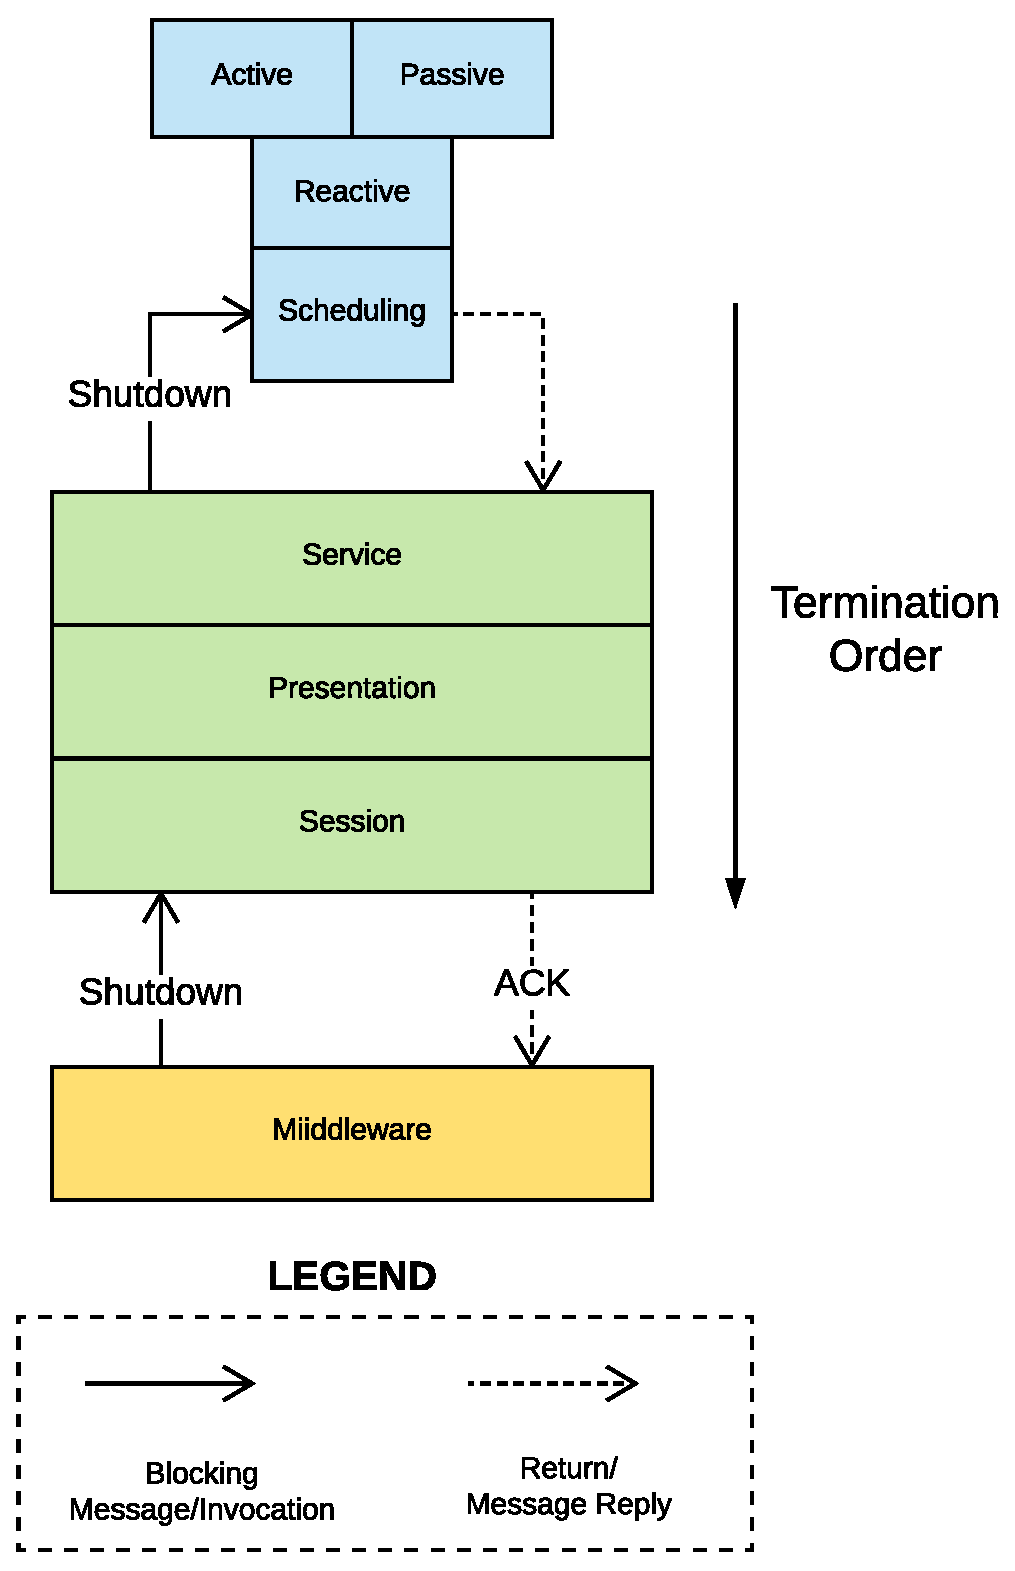
\includegraphics[scale=0.4,keepaspectratio]
    {images/solution/termination-app.eps}
  \caption{Application Termination}
  \label{fig:termination-app}
\end{figure}

%TODO: Review termination process
\begin{enumerate}
  \item The middleware sends a \verb|shutdown| message to IL;
  \item The upwards components\footnote{these components carry the messages
  from middleware to the application layer} of the sublayers of IL terminates
  themselves when they
  read the shutdown request in the header. This is achieved by a transition
  from \verb|active| to \verb|stopped| state, which enables the master
  of each event loop to wait for all its workers to complete. Then the master
  puts the shutdown notification in the queue of the next IL component;
  \item The shutdown message is forwarded upwards until it reaches the Scheduling
  component. Then the scheduler notifies its workers. The workers change their
  state to \verb|stopped| and wait on a barrier until all the other workers have
  completed their execution. \\
  At this stage, we have the guarantee that no worker is running at
  the Application Layer level. Indeed, all the Application Layer
  entities are inerts because their engine (i.e., the scheduler) has been
  turned off;
  \item The previous point implies that we can safely terminate
  also the downwards components of the IL subsytem. Indeed, no message
  will be sent if the scheduler is not running. Thus, as last message
  an acknowledgment to the shutdown request
  originally sent by the middleware is packed
  by the stub component and sent downwards through the IL forwarding pipeline;
  \item All the downwards components of IL behaves exactly as the upwards one;
  \item The sender component forwards the acknowledgment message
  to the middleware.
\end{enumerate}


We implement also a dump method, to enable each stateful entity to save its
state before terminating. However we have not
been able to test it successfully in the distributed environment. Thus, we
kept it in the source code but we did not use it in production.



Similarly to the bootstrap phase, the middleware expects to receive the
\verb|shutdown| ack message within a certain amount of time.
In order to do so, when sending the message, the middleware starts a timeout.
Wherefore if it expires before receiving a response message,
it retransmit again the \verb|shutdown| request towards the application.

\subsubsubsection{Interaction between entities}

The application contains several interactions among entities that have to be
specified in order to understand well how to approach different problems.

\paragraph{Entering a road} Moving entities enter a road by entering a stretch
that is located at the beginning of the road and that is treadable by their
specific entity type.

\paragraph{Entering a road stretch} Moving entities who want to enter a new
road stretch can do it whenever there is room for them in that stretch. In
particular, a roadway stretch can be trod for at most one vehicle at the same
time.

\paragraph{Zebra crossings} Vehicles which want to enter a road stretch that
has zebra crossings painted on it has to wait for pedestrians or bikes to free
all stretches of that particular crossing.

\paragraph{Changing roadway lane} A vehicle that is on the i-th road stretch
which wants to change lane has to wait until the (i+1)-th stretch in the
wanted direction is free.

\paragraph{Crossroads} Every road that is connected to a crossroads is marked
with a cardinal point (N/E/W/S). The crossroads holds all the logic necessary
for vehicles to follow the yield rules we described in
\ref{sec:pa-domain-problems}.

There could be a situation in which there is a standstill, for example when
four cars want all to go straight in a four-way crossroads. In this case, the
crossroads will make a car yield the right-of-way to another one.

Pedestrians can only walk on the corner of the crossroads, thus passing to the
adjacent piece of road (e.g. a pedestrian that is coming from the ``southern''
side of the western road can only enter the southern street on the ``western''
side).

\paragraph{Entering a building} When a moving entity is in the stretch where
there is the entrance of a building, then it may enter the building.

If the moving entity is a vehicle, it has to wait for all other entities who
are in the intermediate stretches to move away.

\paragraph{Exiting a building} When a moving entity is exiting a building, it
has to check whether there is room for her to move out.

If the entity is a vehicle, it has to yield the right-of-way to upcoming
vehicles and to wait that eventual sidewalks or bicycle path stretches in front
of the building are free too.

\paragraph{Choosing to use a vehicle} An entity $e$ who wants to leave a
building $b_e$ to a destination $d_e$ may randomly decide not to travel by
foot. She can leave only if:

\begin{itemize}
  \item the path from $b_e$ to $d_e$ does not include any destination of other
    people who are leaving from $b$ and viceversa. Otherwise, they would share
    the vehicle if there is enough room;
  \item there is an available vehicle in $b_e$; and
  \item the capacity of the destination building $d_e$ is greater than the sum
    of all vehicles in it and the ones which are arriving to that building.
\end{itemize}

If all of these conditions are met, then:
\begin{itemize}
  \item the entity may exit the building and travel using a vehicle; and
  \item $d_e$ now ``books'' a place for the vehicle driven by $e$.
\end{itemize}

\paragraph{Waiting for a bus} A pedestrian may randomly decide to wait for a
bus if she is on a bus stop stretch.

Firstly, she checks whether the buses that stops at that stretch match (even
partially) her path. If at least one of them does, then she wait for a limited
amount of time for a bus to arrive.

If this timeout expires, then she continues travelling by foot to the next
stretch.

\paragraph{Boarding a bus} When a bus arrives at a bus stop, then a waiting
entity will board it only if:

\begin{itemize}
  \item there is enough room for her; and
  \item this bus shortens the expected route for her.
\end{itemize}

\paragraph{Getting off a bus} A person $p$ will get off a bus when it reaches
the last stop $s$ such that $s$ belongs to the route of $p$.

\paragraph{Respecting street code} Roads and crossroads will contain all the
necessary logic to make moving entities follow the street rules.

\paragraph{Performing an overtaking} This action is possible only when a
vehicle is able to change lane. It might be triggered by a timeout which
expires when it is waiting too much for entering the next straightaway stretch.

When a vehicle tries to overtake another one, it will always try to return to
the lane where it started the operation before entering the last stretch.
% look for "manovra" translation

% \paragraph{Uber} % Is it a TODO?




\subsubsection{Middleware}
\subsubsubsection{Application - Middleware}
The communication protocol between application layer and middleware layer 
\paragraph{Fire and forget} 
It is a one-way message pattern (the service sends a message without expecting a response). 
Since the application and the middleware will reside on the same physical node we can assume 
that the communication is reliable, once a message is sent from the application layer it arrives to 
the middleware layer and viceversa.
The asynchronous communication decouples the computation of the application from the 
computation of the middleware and viceversa. The standard interfaces for communication 
implemented by application layer and middleware layer enables the use of etherogenous 
technologies for each one. Defining a standard interface is fundamental to abstract from 
the underlying technologies (implementation).

\subsubsubsection{Middleware - Middleware}


% Distribution - Middleware Layer subsection
\subsection{Distribution -- Middleware layer}
This section presents the services that make up the middleware.

Before seeing every service in detail, it is useful to have an overview to the
organization of those components.

\begin{figure}[H]
  \centering
  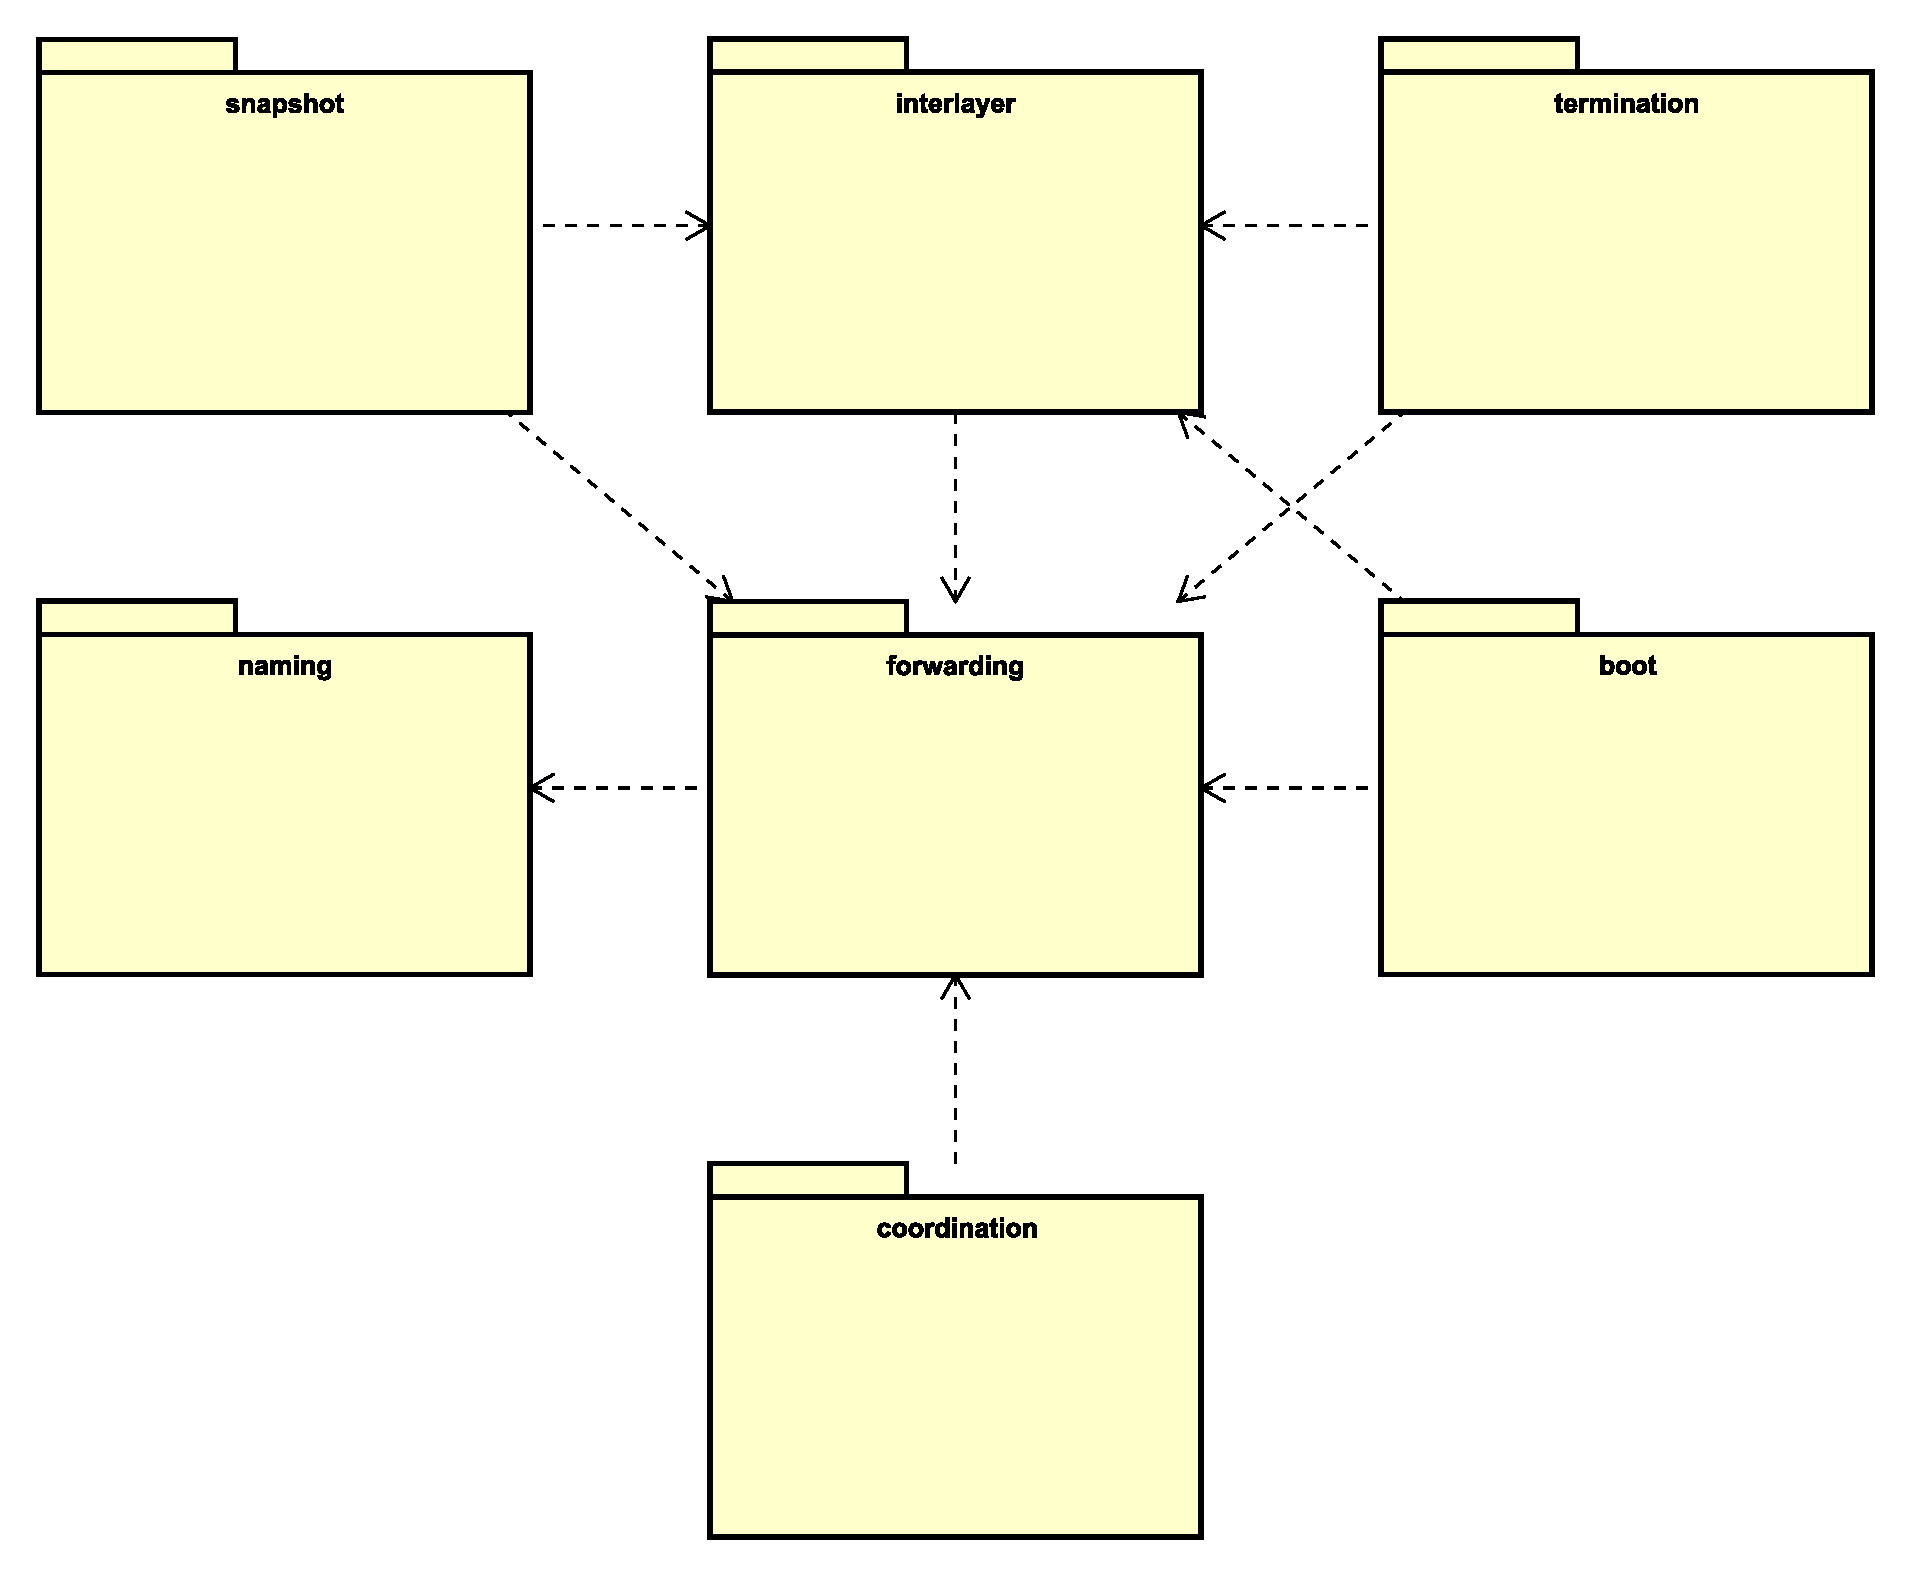
\includegraphics[width=\columnwidth]{images/solution/mw/overview.eps}
  \caption{Middleware architecture overview}
  \label{fig:mw-arch-over}
\end{figure} % TODO: Remove naming package

\begin{itemize}
  \item \texttt{naming}: service that provides a correspondence between logic
    names and their actual location;
  \item \texttt{forwarding}: service that represents the abstraction through
    which it is possible to deliver messages to other middleware nodes;
  \item \texttt{incoming}: service that is responsible of handling messages
    coming from other middleware nodes;
  \item \texttt{interlayer}: service that represents the interface between
    the application and middleware layers;
  \item \texttt{boot}: service that is responsible to start the system neatly;
  \item \texttt{termination}: service that shut downs the node and the system
    gracefully;
  \item \texttt{snapshot}: service that takes consistent views of the node and
    the system;
  \item \texttt{coordination}: service that coordinates the interaction among
    the nodes of the system;
  \item \texttt{persistence}: service that provides a set of utilities to
    store data in a persistent way.
\end{itemize}

\subsubsection{Naming service}
The Naming service, provided with an entity id and its type, finds the node on
which a given entity resides.

This is done in a completely decoupled way with respect to the application
layer, which just provides the identifier and the type of the entity in the
headers of the message handed over to the middleware. Then, the middleware
Naming component will just have to look for this entity in a configuration
file.

\subsubsection{Forwarding service}
The Forwarding service has to deliver messages to other nodes. This component
is very simple, since it just has an interface (\texttt{MQProxy}) and its
implementation, \texttt{RabbitSender}.

Basically, a \texttt{RabbitSender} takes a message as input and guarantees to
send it to the intended recipient, which could be middleware node or a
RabbitMQ pub/sub queue directed to our brokers.
\texttt{RabbitSender}s are able to make this decision by simply looking if the
messages they are handling are events or node-to-node communication. In the
first case (events), messages are propagated towards the frontend of the
application (and therefore to the brokers). In the other case, messages are
just sent to the node the sender finds in the recipient field of the message.

\subsubsubsection{Incoming}
The Incoming application is responsible of receiving messages from other
middleware nodes and to dispatch these messages to the appropriate middleware
application.
However, before dispatching this component process the message by applying some
checks: in fact, a message may be directed to another node or it might have to
be withheld if a snapshot is occurring.

Therefore, we decided to take advantage of Elixir's
\href{https://hexdocs.pm/gen_stage/GenStage.html}{GenStage} behaviour and
structure the modules of this component as a pipeline through which the
message is processed:

\begin{figure}[H]
  \centering
  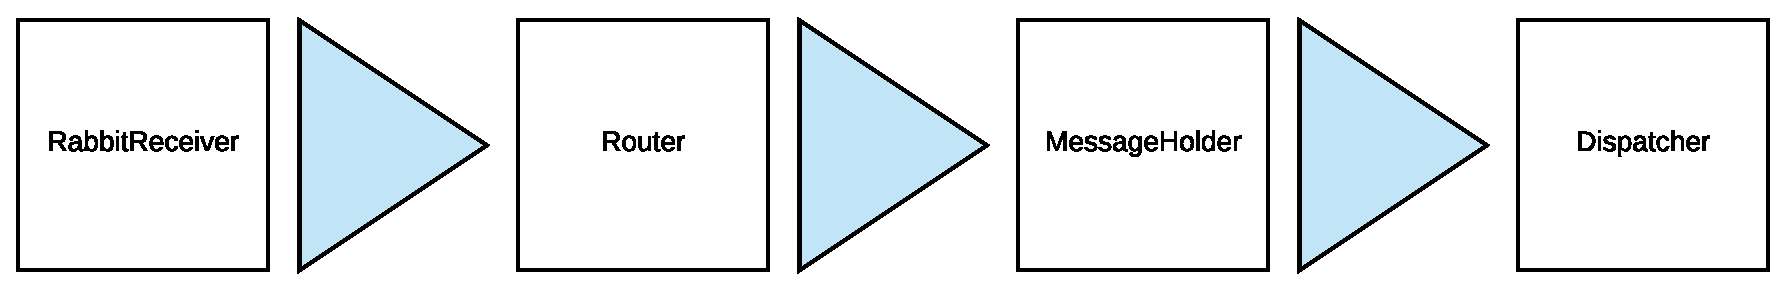
\includegraphics[width=\columnwidth]{images/solution/mw/inc/architect.eps}
  \caption{Incoming pipeline}
  \label{fig:mw-incoming}
\end{figure}

\begin{itemize}
  \item A RabbitReceiver is a process which receives messages from a single
    adjacent middleware node (or ``neighbor'') using RabbitMQ
  \item A Router compares the recipient field of the message with the
    identifier of the current node. If it is different, then it forwards the
    message to the next node along the path to the recipient
  \item A MessageHolder prevents messages to reach the dispatching point if a
    snapshot is happening. Then, when the snapshot ends, the messages will be
    forwarded again towards the Dispatcher
  \item A Dispatcher dispatches messages to a given application of the middleware
\end{itemize}

\begin{figure}[H]
  \centering
  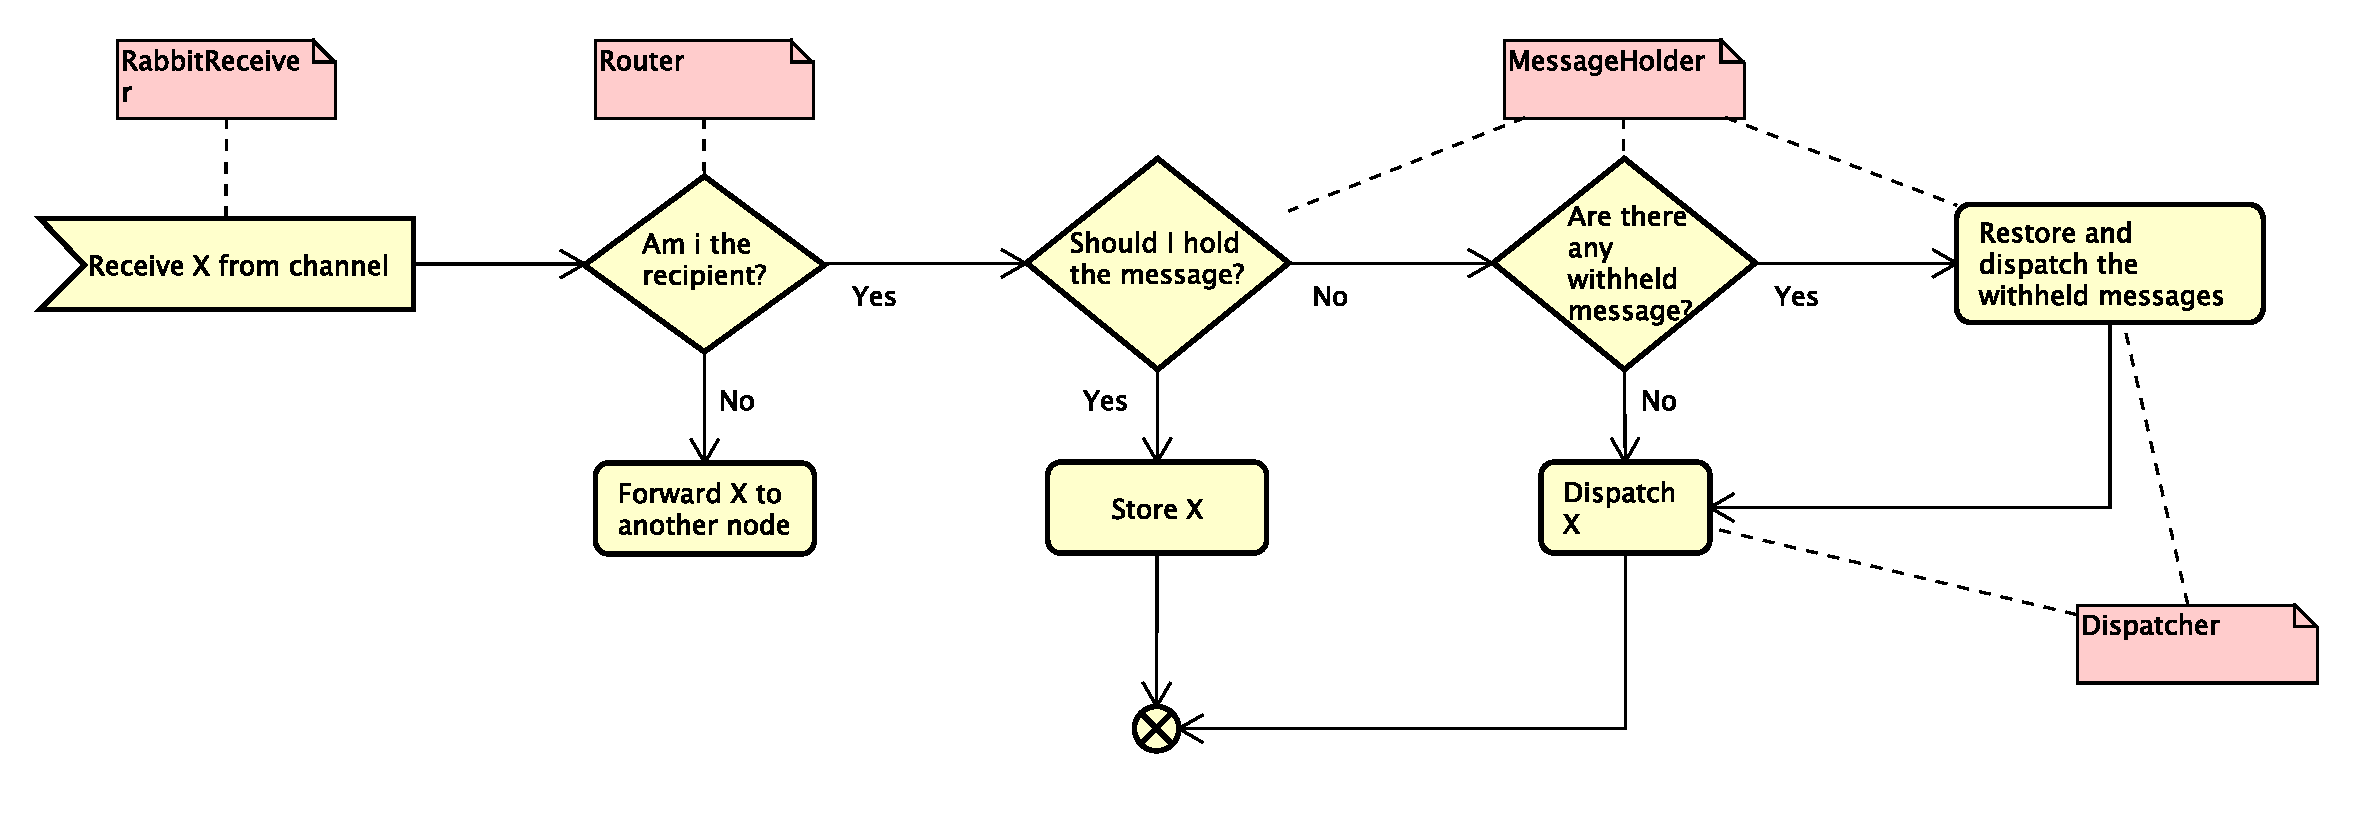
\includegraphics[width=\columnwidth]{images/solution/mw/inc/activity.eps}
  \caption{Activity diagram for Incoming pipeline}
  \label{fig:mw-incoming-activity}
\end{figure}

Thanks to the flexibility of GenStage, we can compose our pipelines by adding
an arbitrary number of elements at each stage of the pipeline. For instance,
there is one RabbitReceiver for each middleware neighbor plus one for loopback
communication: in this case, we just have to spawn as many RabbitReceivers as
needed and then make the Router subscribe to the events generated by them
(that is, the incoming messages).

\subsubsection{Interlayer service}

This component is responsible of the communication that is performed among
different layers, namely the one which it belongs (the \textbf{middleware}) and
another one who uses the middleware layer, that is the \textbf{application}
layer.

We show in figure \ref{fig:mw-interlayer} the architecture of this service and
then we will show in detail each module that composes this component.

\begin{figure}[H]
  \centering
  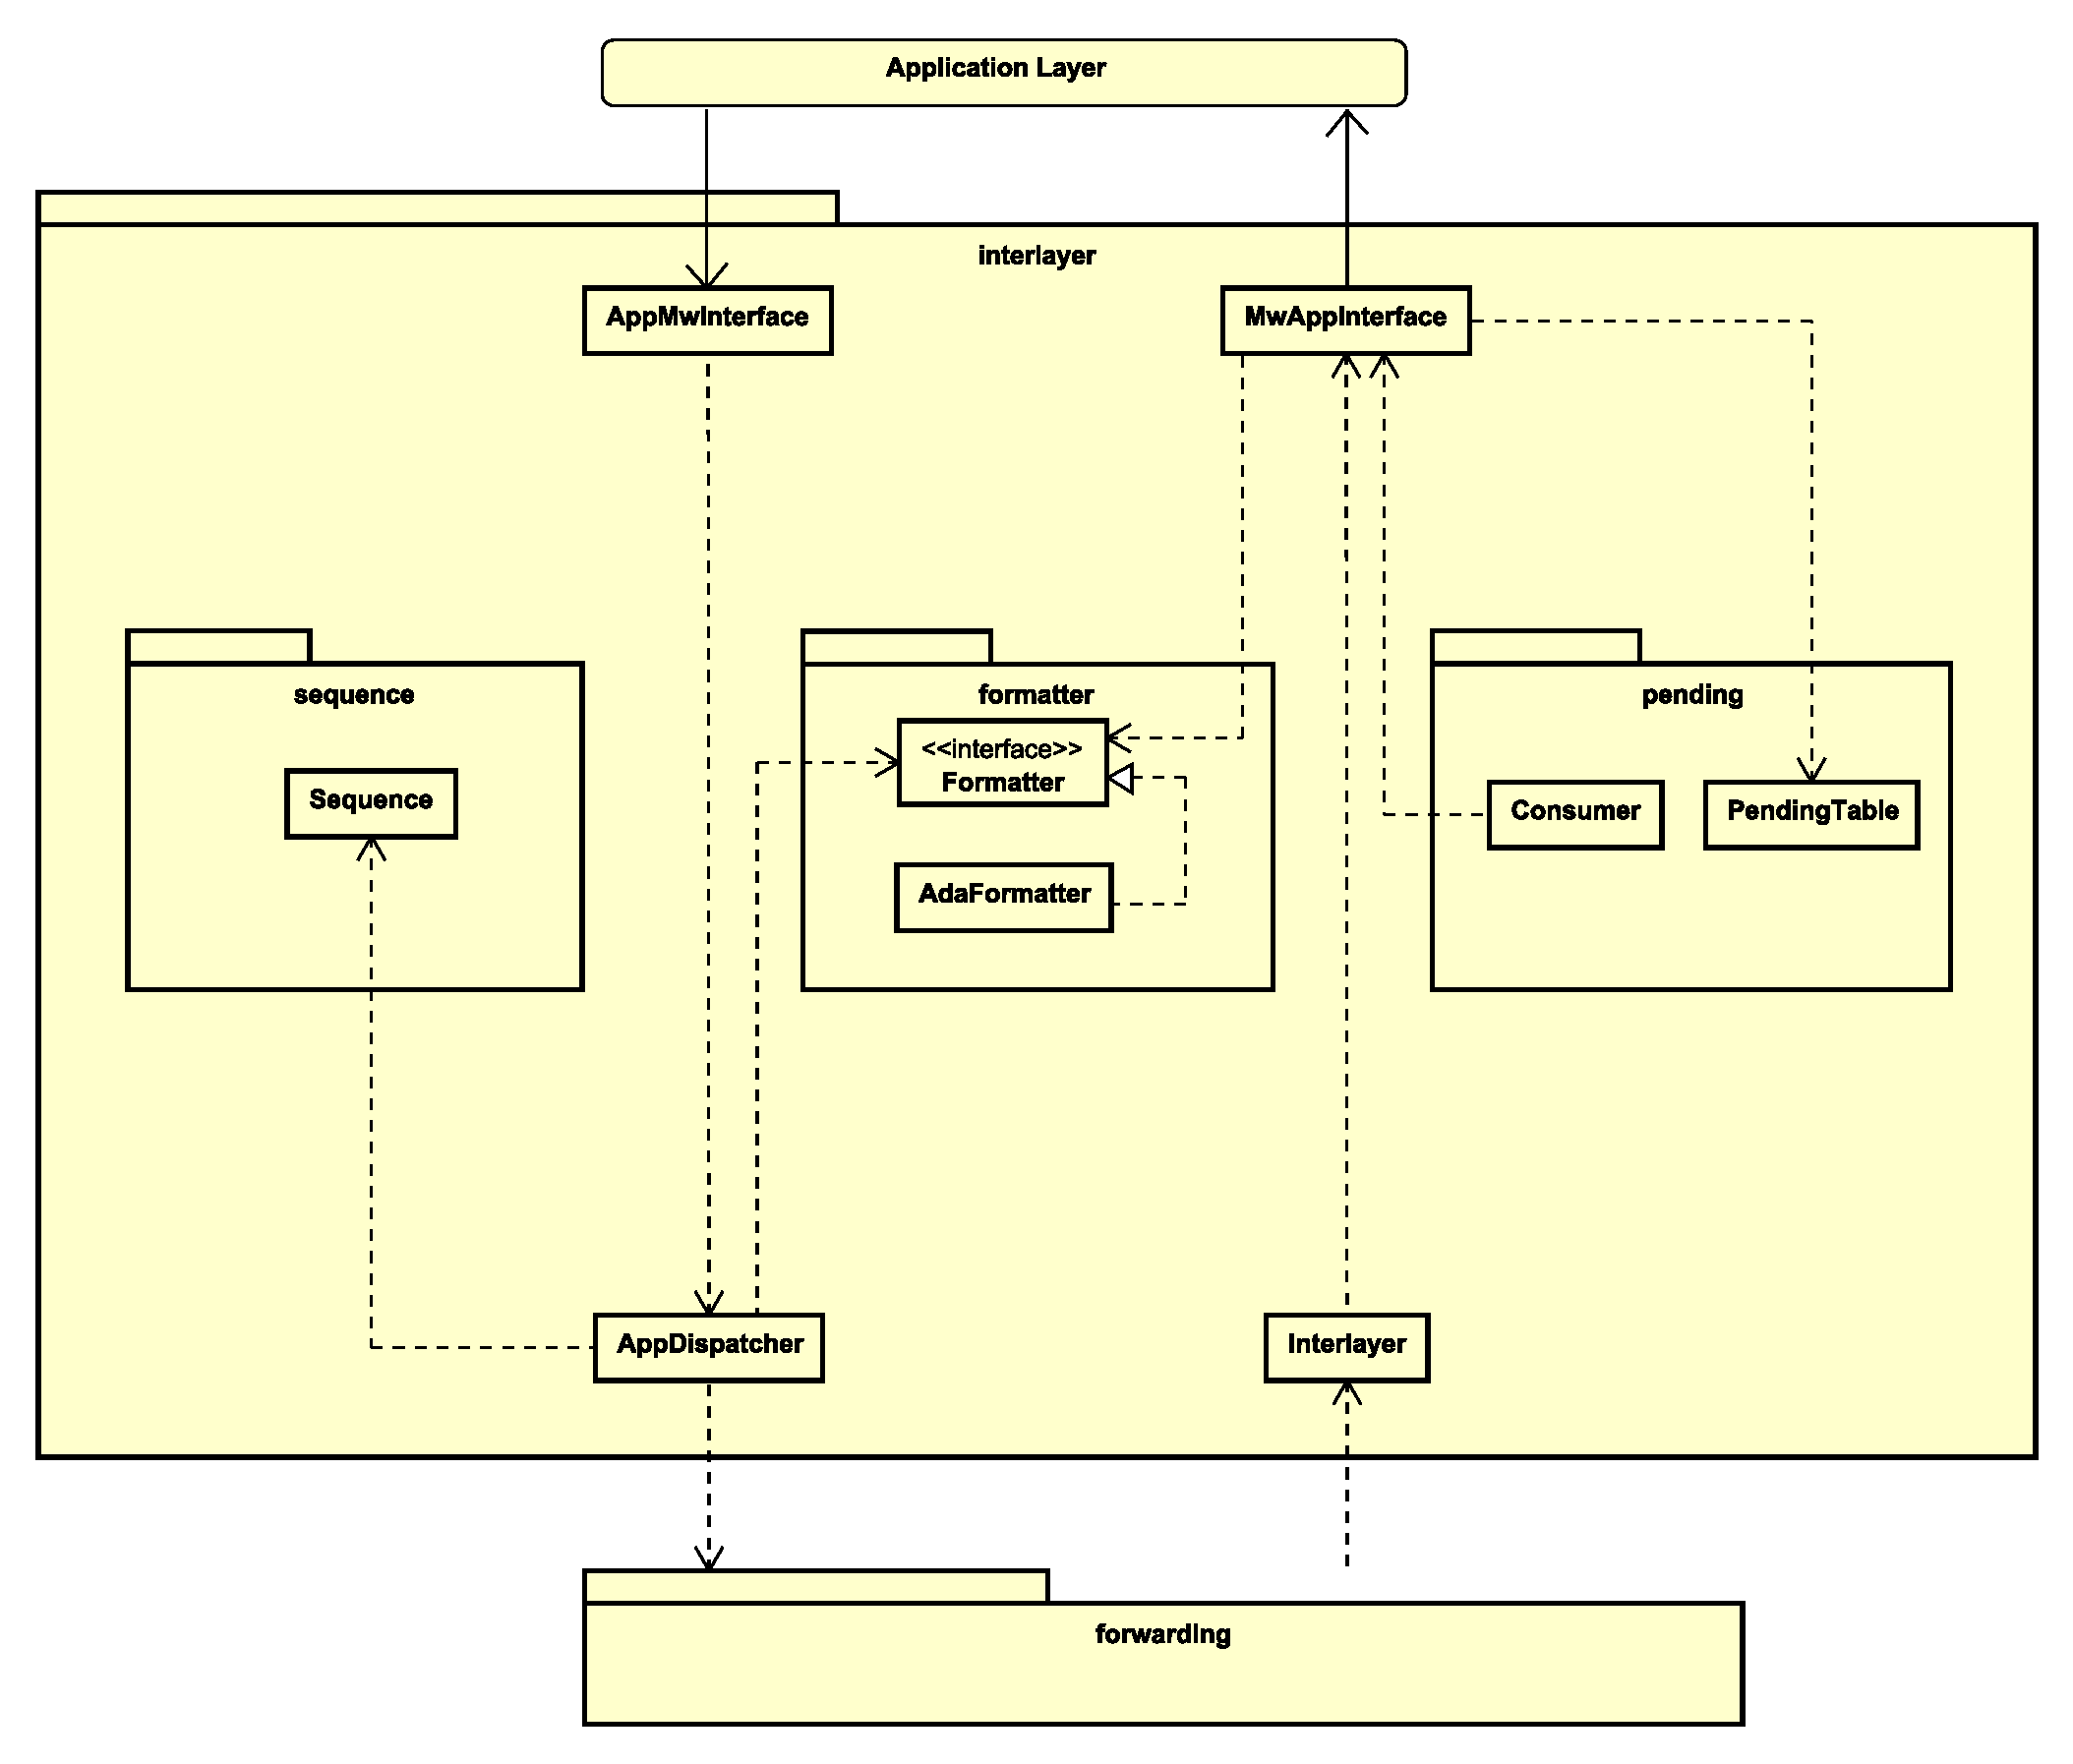
\includegraphics[width=\columnwidth]{images/solution/mw/interlayer.eps}
  \caption{Middleware's Interlayer service}
  \label{fig:mw-interlayer}
\end{figure} % TODO: needs update (Sequence usage comes from AppMwInterface)

% TODO: All class diagrams has to be added
\subsubsubsection{interlayer.Interlayer}

\subsubsubsection{interlayer.MwAppInterface}

\subsubsubsection{interlayer.AppMwInterface}

\subsubsubsection{interlayer.AppDispatcher}

\subsubsubsection{interlayer.sequence.Sequence}

\subsubsubsection{interlayer.formatter.Formatter}

\subsubsubsection{interlayer.formatter.AdaFormatter}

\subsubsubsection{interlayer.pending.PendingTable}

\subsubsubsection{interlayer.pending.Consumer}

\subsubsection{Boot service}\label{sec:mw-boot-descr}

The Boot service is responsible of starting the system in a graceful fashion.
It does so by dividing the start phase into two subphases, namely the
\textbf{marker diffusion} and the \textbf{(own) boot} phase. The procedure is
the same shown in Figure \ref{fig:sys-bootstrap-protocol}, with the first phase
going from left to right and the second phase going in the opposite direction.

In this context, by \textit{marker} we will mean \textit{boot marker}.

When receiving a marker, this the Boot service will forward the marker to all
of its adjacent middleware nodes.
Then, when receiving further markers, this service will just reply immediately
with an end marker.

After having received all the replies for the markers, the Boot service will
request to the application layer to gracefully start.
When the application layer will inform the middleware it started, this service
will send an end marker to all of its adjacent middleware nodes.

\subsubsection{Termination service}

The Termination service is responsible of shutting down the system gracefully.
It does in a symmetrical way to what we have seen in Section
\ref{sec:mw-boot-descr} for the Boot service.

Initially, this service is in a \texttt{running} state, which means the
application layer is normally running.

If the middleware receives a stop marker, it will forward the request marker to
all of its neighbors and any of the subsequent incoming request markers will
receive an immediate reply to fulfill the request.

Then, when the Termination service receives all the replies for the stop marker
from its neighbors, it will send a reply back for the stop request marker and
enter a \texttt{terminating} state, sending an asynchronous request to the
application to stop.

During this second phase, the middleware will wait for a termination marker.
When it arrives, it will forward the termination request marker to all of its
neighbors and reply immediately to any other termination request marker which
arrives by fulfilling it.

As soon as the application will inform the middleware layer that the former is
stopped, the latter will enter a \texttt{stopped} state.

The Termination service will wait both for all of the neighbors to send back a
reply to the termination marker and for itself to enter the \texttt{stopped}
state.
After this, the node will send back a reply for the termination request, ending
the termination procedure for the current node and entering the
\texttt{terminated} state.

%TODO: Add picture

\subsubsection{Snapshot service}
This component is responsible of taking snapshots.

We show in figure \ref{fig:mw-snapshot} the architecture of this service and
then we will show in detail each module that composes this component.

\begin{figure}[H]
  \centering
  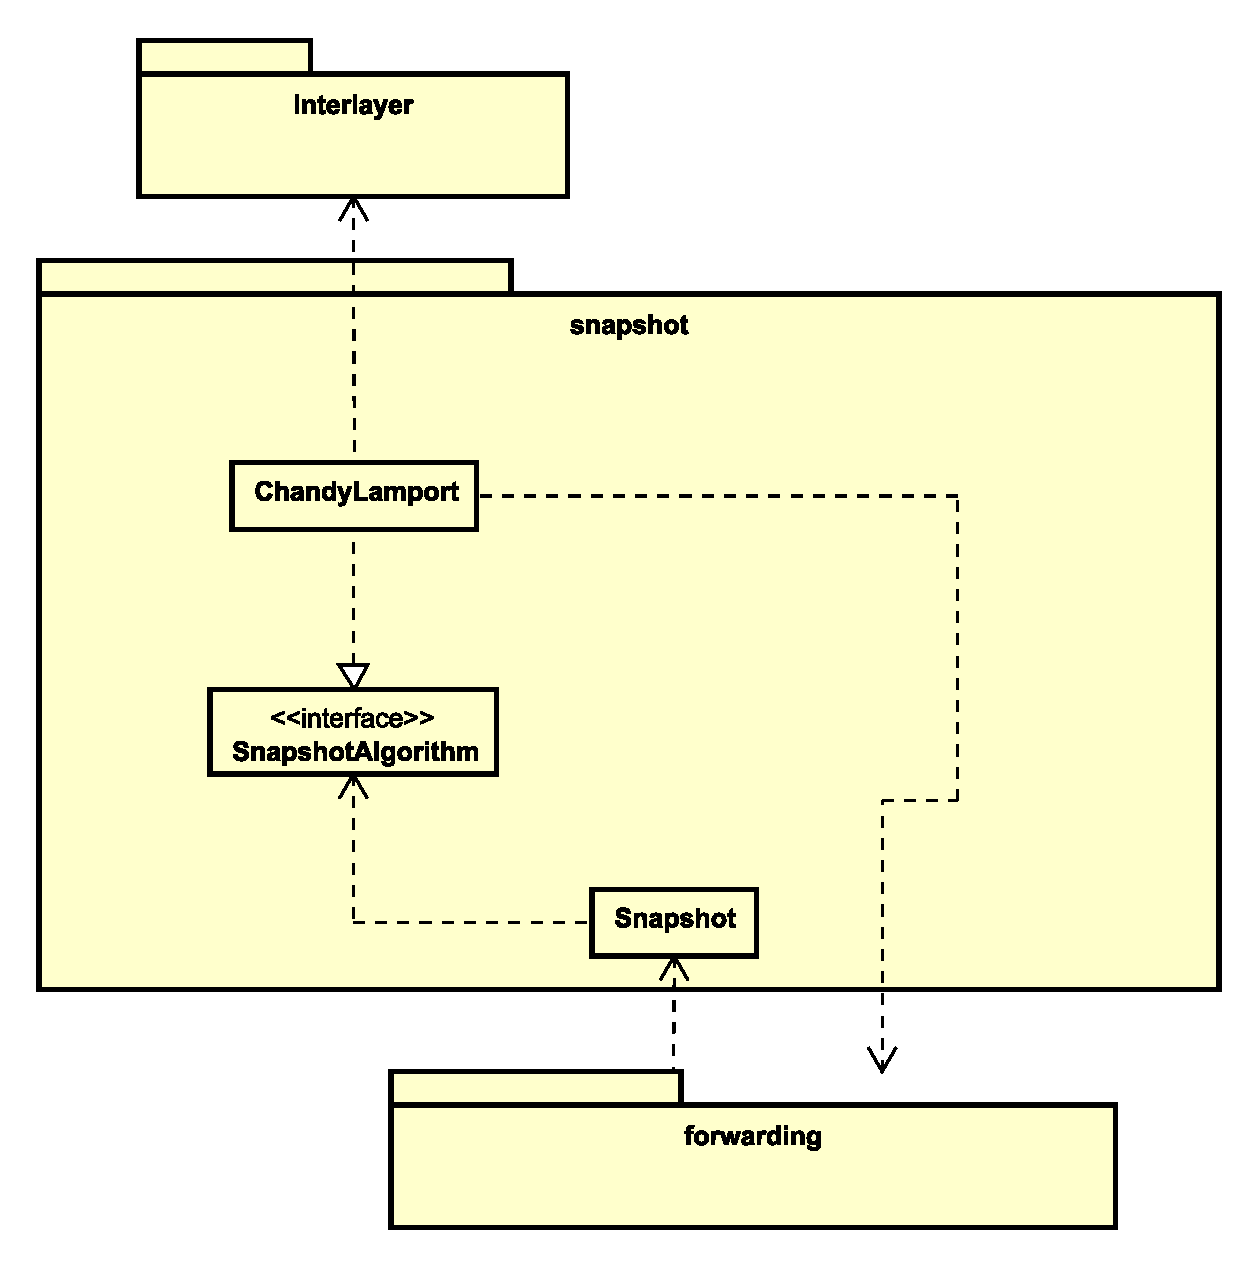
\includegraphics[width=\columnwidth]{images/solution/mw/snapshot.eps}
  \caption{Middleware's Snapshot service}
  \label{fig:mw-snapshot}
\end{figure}

% TODO: All class diagrams have to be added
\subsubsubsection{snapshot.Snapshot}
% TODO: Class diagram
\FloatBarrier
\begin{itemize}
  \item \textbf{Description} \\
    This module is the Fa\c cade of the Snapshot service. It is responsible
    to boot neatly and supervise all processes in Snapshot. Also, it has to
    handle snapshot requests that come from other nodes of the system.
  \item \textbf{Attributes}
  \item \textbf{Operations}
  \begin{itemize}
    \item \texttt{+ start()} \\
    Starts the Snapshot service.
    \item \texttt{+ handleMessage(message: String)} \\
    % TODO: check this out: Message will really be a String?
    Handles a snapshot start/termination request that comes from other nodes
    or receives snapshot information from the application layer.
  \end{itemize}
\end{itemize}

\subsubsubsection{snapshot.SnapshotAlgorithm}
% TODO: Class diagram
\FloatBarrier
\begin{itemize}
  \item \textbf{Description} \\
    Interface for processes that implement a certain kind of snapshot.
  \item \textbf{Attributes}
  \item \textbf{Operations}
  \begin{itemize}
    \item \texttt{+ take()} \\
    Starts to take a snapshot.
    \item \texttt{+ submitLocalSnapshot()} \\
    Stores a local snapshot.
    \item \texttt{+ submitRemoteSnapshot()} \\
    Stores a remote snapshot.
  \end{itemize}
\end{itemize}

\subsubsubsection{snapshot.ChandyLamport}
% TODO: Class diagram
\FloatBarrier
\begin{itemize}
  \item \textbf{Description} \\
    Module that implements the \texttt{snapshot.SnapshotAlgorithm}
    interface to take snapshots with the algorithm by Chandy and Lamport.
  \item \textbf{Attributes}
  \item \textbf{Operations}
  \begin{itemize}
    \item \texttt{+ take()} \\
    Starts to take a snapshot: that implies Forwarding module to notify
    other nodes of that and to hold messages until the snapshot is over; also
    that implies Interlayer to issue a snapshot request to the application
    layer.
    \item \texttt{+ submitLocalSnapshot()} \\
    Stores the snapshot of the node where the process is executing.
    \item \texttt{+ submitRemoteSnapshot()} \\
    Stores the snapshot of a remote node.
  \end{itemize}
\end{itemize}

\subsubsection{Coordination service}

This component is responsible of the coordinating middleware nodes by
providing mechanisms with which the system is able to operate cohesively.

We show in figure \ref{fig:mw-coordination} the architecture of this service
and then we will show in detail each module that composes this component.

%\begin{figure}[H]
%  \centering
%  \includegraphics[width=\columnwidth]{images/solution/mw/coordination.eps}
%  \caption{Middleware's Coordination service}
%  \label{fig:mw-coordination}
%\end{figure}
% TODO: Add diagram

% TODO: All class diagrams have to be added
\subsubsubsection{coordination.Coordination}
% TODO: Class diagram
\FloatBarrier
\begin{itemize}
  \item \textbf{Description} \\
    This module is the Fa\c cade of the Coordination service. It is responsible
    to boot neatly and supervise all processes in Coordination.
  \item \textbf{Attributes}
  \item \textbf{Operations}
  \begin{itemize}
    \item \texttt{+ start()} \\
    Starts the Coordination service.
    \item \texttt{+ handleMessage(message: String)} \\
    % TODO: check this out: Message will really be a String?
    Receives a message and delegates the proper handling of it to an internal
    module.
  \end{itemize}
\end{itemize}

\subsubsubsection{coordination.coordinationInfo}
% TODO: Class diagram
\FloatBarrier
\begin{itemize}
  \item \textbf{Description} \\
    Process that holds the current state of the coordination.
  \item \textbf{Attributes}
    \begin{itemize}
      \item \texttt{- state: Map<Atom,Any>} \\
    Information about coordination.
    \end{itemize}
  \item \textbf{Operations}
  \begin{itemize}
    \item \texttt{+ startLink()} \\
    Starts the process and initialize \texttt{state} as an empty map.
    \item \texttt{+ getInfo(key: Atom)} \\
    Returns the information contained in the state at the entry \texttt{key}.
    \item \texttt{+ setInfo(key: Atom, value: Any)} \\
    Modifies the state held by the process by setting the entry \texttt{key}
    to the value \texttt{value}.
  \end{itemize}
\end{itemize}

\subsubsubsection{coordination.election.Election}
% TODO: Class diagram
% TODO: Explode class in interface and implementation
\FloatBarrier
\begin{itemize}
  \item \textbf{Description} \\
    Process that is responsible to manage the election of a system coordinator.
  \item \textbf{Attributes}
    % TODO
  \item \textbf{Operations}
    % TODO
\end{itemize}

\subsubsubsection{coordination.time.HeartbeatMaker}
% TODO: Class diagram
\FloatBarrier
\begin{itemize}
  \item \textbf{Description} \\
    Process that has to produce an heartbeat (i.e., a signal that represents
    the logical clock ticking in the system) for all the nodes in the
    system.
  \item \textbf{Attributes}
  \item \textbf{Operations}
  \begin{itemize}
    \item \texttt{+ start()} \\
    Starts HeartbeatMaker process.
    \item \texttt{+ enable()} \\
    Makes HeartbeatMaker begin producing heartbeats.
    \item \texttt{+ disable()} \\
    Makes HeartbeatMaker stop producing heartbeats.
  \end{itemize}
\end{itemize}

\subsubsubsection{coordination.time.HeartbeatListener}
% TODO: Class diagram
\FloatBarrier
\begin{itemize}
  \item \textbf{Description} \\
    Process that listens to heartbeats. It is responsible to delivering them
    to the application layer.
  \item \textbf{Attributes}
  \item \textbf{Operations}
  \begin{itemize}
    \item \texttt{+ start()} \\
    Starts HeartbeatListener process.
    \item \texttt{+ beat()} \\
    Notifies the application layer of a new heartbeat.
  \end{itemize}
\end{itemize}



% Concurrency - Application Layer subsection
\subsection{Concurrency - Application Layer}
This section presents the concurrent entities forming the application layer of the system.
\paragraph{Types of entities}
Three types of entities have been identified
\begin{itemize}
  \item \textit{Active}: an entity capable to start an action by itself, 
  providing it the computational resources it needs;
  \item \textit{Reactive}: an entity with an inner state, that only acts on reaction to external inputs, 
  and it is not capable to start an action by itself;
  \item \textit{Passive}: an entity with an internal state (if necessary) which is immutable. 
   As a Reactive entity It only acts on reaction to external inputs, and it is not capable to start an action by itself.
\end{itemize}
\begin{table}[H]
\centering
\begin{tabular}{|l|l|}
\hline
\rowcolor{BlueGreen}
Type     & Entities                                 \\ \hline
Active   & pedestrian, bicycle, motorcycle, car, bus, semaphore \\ \hline
Reactive & road, crossroads, sidewalk, bike lane, crossing, house \\ \hline
Passive  & road signs                               \\ \hline
\end{tabular}
\caption{Types of entities}
\label{tab:entity_type}
\end{table}
The entities have the following dependencies:
\begin{itemize}
  \item \textit{Active} provides inputs to \textit{Reactive} (solid line);
  \item \textit{Active} and \textit{Reactive} can use \textit{Passive}, the dependency is not strict (dashed line).
\end{itemize}
\begin{figure}[H]
  \centering
  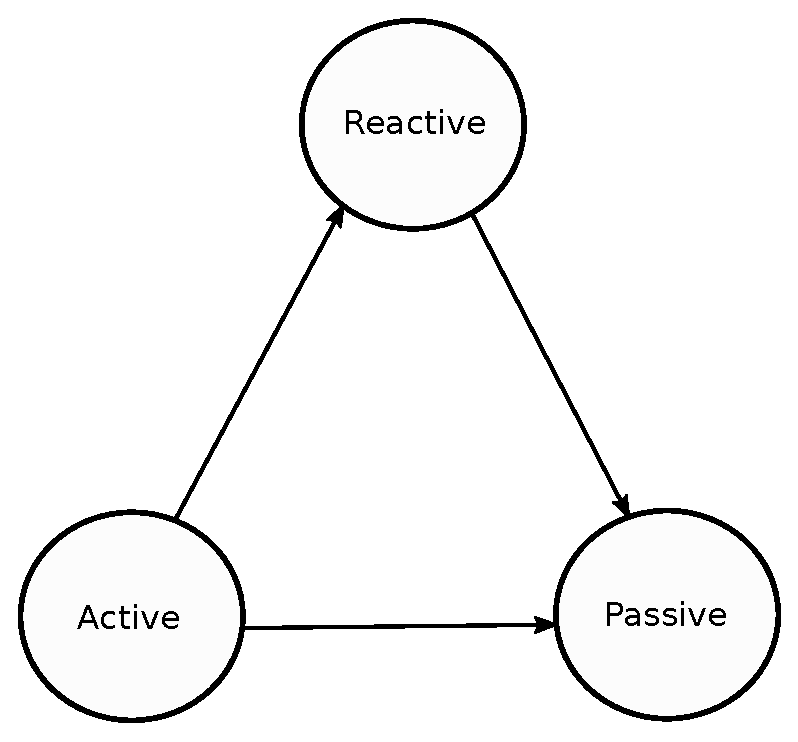
\includegraphics[width=.35\columnwidth]{sections/images/solution/entity_type_dependency.eps}
  \caption{Dependencies between entity types}
  \label{fig:sd-entity-types-deps}
\end{figure}

\subsubsection{Architectural Design}
Overview of the application layer: the classes have been divided according to 
\ref{tab:entity_type}.
\begin{figure}[H]
  \centering
  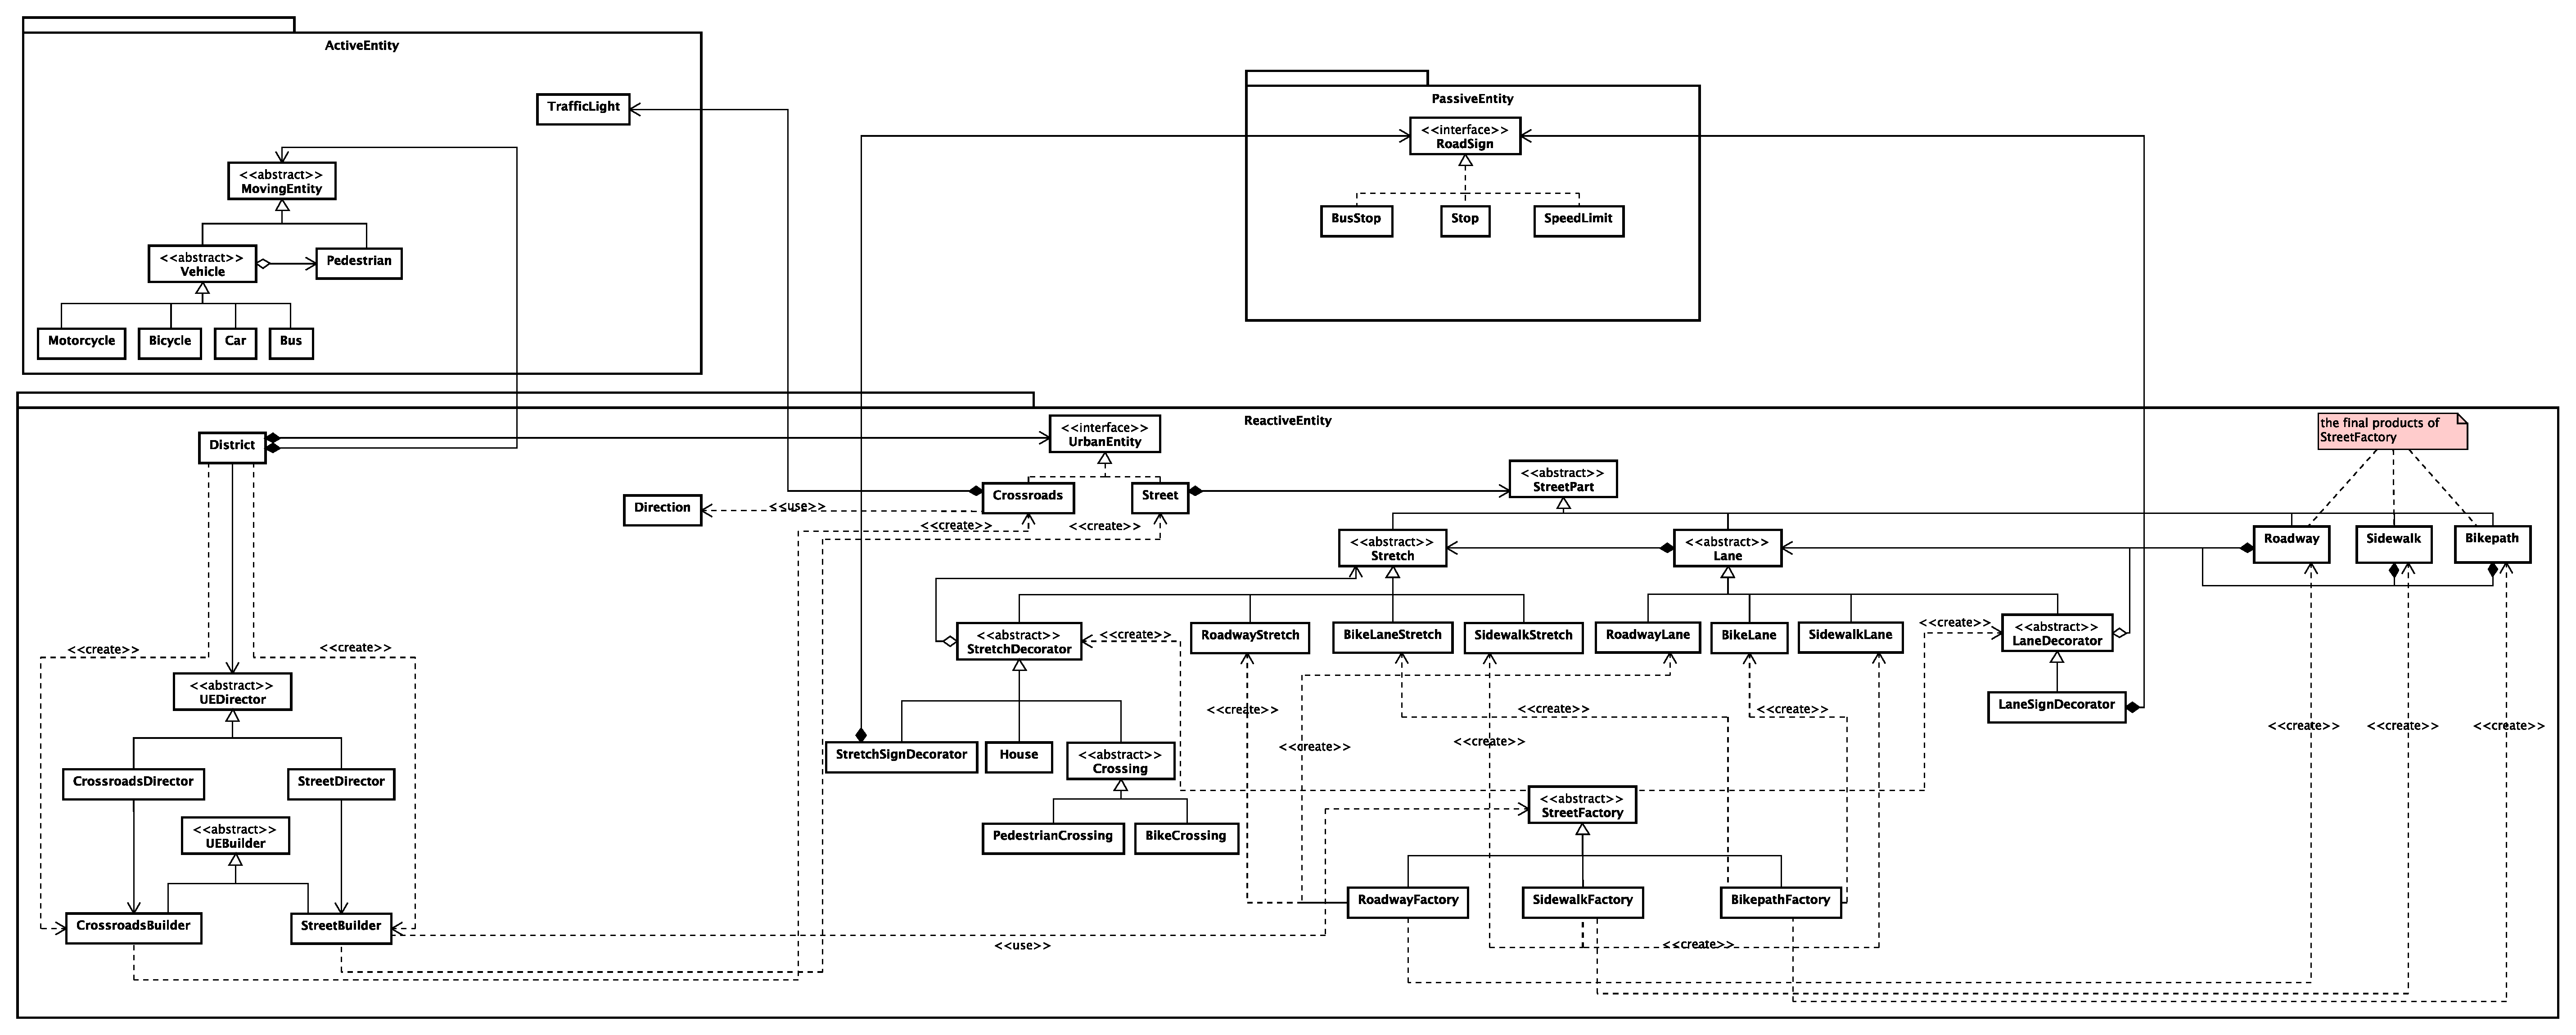
\includegraphics[width=.95\columnwidth]{images/solution/app_architecture.eps}
  \caption{Application Layer: top level design}
  \label{fig:sd-app-architecture}
\end{figure}


\subsubsection{Road}
\begin{figure}[h]
\centering
\nogloxy{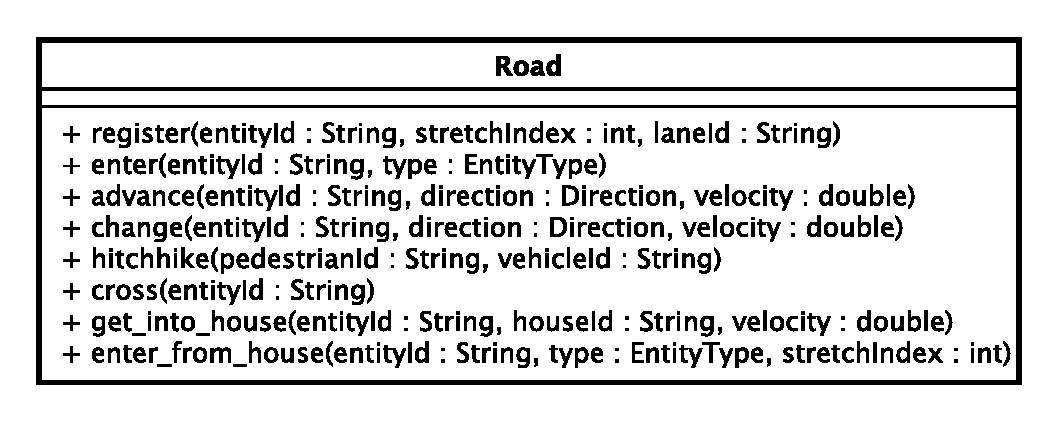
\includegraphics[scale=0.6,keepaspectratio]{diagrams/workspace/application/road.eps}}
\caption{Application::Road}
\end{figure}
\FloatBarrier
A Road is made of stretches and it offers the following operations:
\begin{itemize}
	\item \texttt{register(entityId : String, stretchIndex : int, laneId : String)}
	\\Puts an entity into the stretch having the given index
	\begin{itemize}
		\item \textit{Use}: boostrap phase
	\end{itemize}
	\item \texttt{enter(entityId : String, type : EntityType)}
	\\Puts an entity into the Road in the rightmost lane available for the entity type
	\begin{itemize}
		\item E.g. a car does not land in a sidewalk
	\end{itemize}
	\item \texttt{advance(entityId : String, direction : Direction, velocity : double)}
	\\Moves an entity forward along the Road	
	\begin{itemize}
		\item If a Road end has reached, the entity is notified providing it the adjacent Roads list
		\item The entity velocity is calculated by each stretch taking a specific range of possible values according to the entity type
	\end{itemize}
	\item \texttt{change(entityId : String, direction : Direction, velocity : double)}
	\\Moves an entity to next stretch in the given direction (left or right)	
	\begin{itemize}
		\item If a Road end is reached, it does not allow the lane change and it sends a message for notifying the entity
		\item If no more lanes for the entity type exist in the given direction, it sends a message for notifying the entity
	\end{itemize}
	\item \texttt{hitchhike(pedestrianId : String, vehicleId : String)}
	\\Brings a pedestrian into an vehicle
	\item \texttt{cross(entityId : String)}
	\\Moves a pedestrian or a cyclist to the other side of the Road
	\begin{itemize}
		\item If there is an entity in the stretch near a sidewalk, it books a Road crossing
		\item No vehicles can enter stretches covered by booked zebra crossing
		\item If a stretch near a sidewalk is free (whether it is booked or not), pedestrian can start crossing the Road
	\end{itemize}
	\item \texttt{get\_into\_house(entityId : String, houseId : String, velocity : double)}
	\\Brings an entity into a house accessible from the Road where the entity is
	\begin{itemize}
		\item It brings the entity into the house, if the entity is in a stretch where the given house is accessible. Otherwise, It moves the entity forward at the specified velocity
	\end{itemize}
	\item \texttt{enter\_from\_house(entityId : String, type : EntityType, stretchIndex : int)}
	\\Brings an entity out from a house and it puts the entity into the Road stretch having the given index
	\begin{itemize}
		\item An entity coming out from a house has lower priority than one is already on the Road. So that, before exiting the house, the first one has to wait the other one is passed
	\end{itemize}
\end{itemize}
\paragraph{Remarks}
\ \\A lane change can happen in two cases:
\begin{itemize}
	\item Overtaking. It is requested in a particular stretch
	\item Road change. It is requested in the first stretch of the Road taken
\end{itemize}
We assume a Road is at least $n$ stretches long if it consists of $n$ lanes for motor vehicles.
\subsubsection{Semaphore}
A semaphore is placed at the end of a road stretch that offers the following functional channels:
\begin{itemize}
	\item \texttt{stop(way)}
	\\Blocks outgoing flow of vehicles going towards a given way
	\item \texttt{yield(way)}
	\\Slows outgoing flow of vehicles going towards a given way	
	\item \texttt{go(way)}
	\\Allows outgoing flow of vehicles going towards a given way
\end{itemize}
Notes:
\texttt{stop}, \texttt{yield} and \texttt{go} are likely to be called by a set of semaphores.
A set of semaphores communicate internally to advance through their RGY steps.
way parameter might be N/S (“vertical” street) or W/E (“horizontal” street).
%\subsubsection{Moving entity}
%TODO add Moving entity section
\subsubsection{House}
\begin{figure}[h]
\centering
\nogloxy{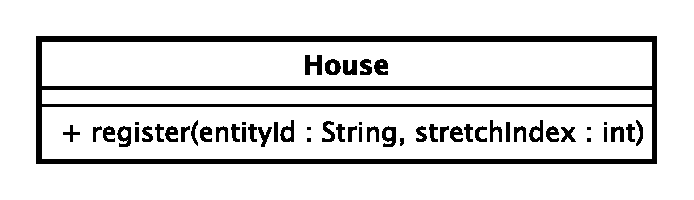
\includegraphics[scale=0.6,keepaspectratio]{diagrams/workspace/application/house.eps}}
\caption{Application::House}
\end{figure}
\FloatBarrier
A house is populated by people and it offers the following operations:
\begin{itemize}
	\item \texttt{register(entityId : String)}
	\\Puts an entity into a house
	\begin{itemize}
		\item \textit{Use}: bootstrap phase
		\item An house defines stocastically the residence time of an entity within it. After freezing, an entity has only the remaining time
	\end{itemize}
\end{itemize}
\subsubsection{Crossroads}
\begin{figure}[h]
\centering
\nogloxy{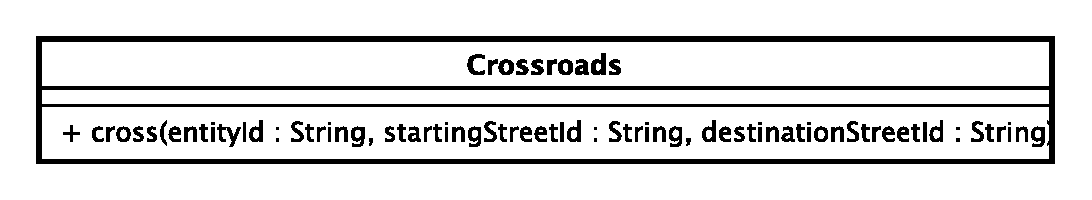
\includegraphics[scale=0.6,keepaspectratio]{diagrams/workspace/application/crossroads.eps}}
\caption{Application::Crossroads}
\end{figure}
\FloatBarrier
A crossroads is a road intersection offers the following operations:
\begin{itemize}
	\item \texttt{cross(entityId : String, startingStreetId : String, destinationStreetId : String)}
	\\Moves an entity from a street to another one
\end{itemize}
%Crossroads’ operations called by entities or roads.
\paragraph{Remarks}
\ \\A crossroads internally encapsulates the logic allows the entities to proceed neatly, i.e. way rules.
%%%%%%%%%%%%%%%%%%%%%%%%%%%%%%%%
%% CONCURRENCY
%%%%%%%%%%%%%%%%%%%%%%%%%%%%%%%%

\subsubsection{Solution to Concurrency Problems}

Our solution addresses the problems we pointed out in section
\ref{sec:pa-concurrency}.
Therefore here we are providing details on how we tackled the questions we
made ourselves at the beginning of the development.

\paragraph{How can we recognize that a situation is suitable to present
concurrency?}
There are several active entities in our application: pedestrians, cars, bikes
and buses. They act because of their own initiative, so they are likely to be
considered as active tasks.

Moreover, their actions cause side-effects to reactive entities like roads.
Consequently our application needs to embody concurrency, i.e., potential
parallelism.

\paragraph{How concurrent accesses will be managed? Will it make sense to
discern side-effect accesses (procedures) from read-only accesses
(\textit{functions})?}
Concurrent accesses will be managed by means of \textit{Protected Objects},
i.e., resources that can be accessed in concurrent read \textbf{or} mutual
exclusive write mode.

It indeed makes sense to have the mentioned separation.
It may be useful to modify roads' status when vehicles travel over them.
On the other hand, it might be useful to get information from them when
someone asks for it without causing side-effects, and this should be doable in
parallel.

\paragraph{Which entities have to be active?}
In light of the fact that active entities undertake spontaneous actions, in
our context they are:
\begin{itemize}
  \item Moving entities, which move around the city according to their own
    will;
  \item Semaphores, which autonomously change their color by the time elapses.
\end{itemize}

\paragraph{Which entities have to be reactive?}
Streets (and all their parts) and crossroads should be reactive entities:
\begin{itemize}
  \item A street is used to travel towards a destination and it is used only
    when it is trod.
    However, the state of a road is composed of the states of the reactive
    sub-entities it comprises, e.g., stretches and houses;
  \item A crossroads coordinates the traffic at street intersections
    exclusively whenever a moving entity requires to cross it.
\end{itemize}

\paragraph{Which entities have to be passive?}
Passive entities are stateless. Therefore, road signs fit perfectly in this
definition, since they represent immutable information that is read by road
users.

\paragraph{Should we use any formal technique to proof the correctness
of the system properties relating to concurrence?}
We will strive to motivate the correctness of our application but we
deliberately do not choose any specific technique.
We did some concurrent tests, that is scheduling tests. In these tests we prove
that executors can start, distribute work across several worker threads and
stop gracefully.

\paragraph{Do we have the possibility to incur a non-valid state?
If so, how do we handle the problem?}
The application will be designed to avoid non-valid states.
However, if the system recognizes it is in a non-valid state, it resumes the
execution from the last valid snapshot.
% resumes: see https://www.cs.york.ac.uk/rts/books/RTSbookThirdEdition/chap6.pdf

\paragraph{How can we avoid possible starvation scenarios?}
The application will be designed to overcome starvation or deadlock scenarios.

In fact, active entities do not hold locks on protected objects and do not
block on RPCs: while the first condition is quite easy to achieve (the
compiler came in to give us a hand), the latter has been not straightforward
to implement.

We designed an event loop which resembles the one present in NodeJS: when
performing an RPC, a worker thread will provide a couple of callbacks (one for
the success case and the other for the failure case): after having instantiated
these callbacks, the thread will be free to execute other active entities,
without awaiting the response.
Clearly, since Ada does not provide enhanced support for closures, we had to
find a way to obtain the same semantics. We did so by defining an interface
\texttt{Callback}, which exposes a single operation, \texttt{Execute} (which
in turn takes no parameters). At this point we just have to concretize
\texttt{Callback} with an appropriate behaviour (e.g., an example of this can
be found in \texttt{Scheduling.Remote.Callback.Success.Tread}).
Actually, the hierarchy we set up is a bit different, since we also added two
intermediate interfaces \texttt{Callback.Success} and
\texttt{Callback.Failure}, in order to use strong typing for pairs of
callbacks.

%%%%%%%%%%%%%%%%%%%%%%%%%%%%%%%%
%% APPLICATION
%%%%%%%%%%%%%%%%%%%%%%%%%%%%%%%%

\subsubsection{Solution to Application Problems}

In section \ref{sec:pa-app-problems} some problems inherently related to the
application domain are explained, and our solution design is thought to solve
them.

\paragraph{Pedestrian Deadlock}
This problem will be avoided ``by design'' by organizing sidewalks in
\textit{lanes}. Though sidewalks in real world usually do not have lanes (apart
from seldom exceptions), we employ the concept of a \textit{logic} lane, i.e.
an abstraction that allows us to coordinate opposite flows of pedestrians in an
agile way.

Since pedestrians proceeding in opposite directions will not compete to enter
the same sidewalk stretch, there can not be any pedestrian deadlock.

\paragraph{Rear-end Collisions}
If the next road stretch of a moving entity route is already taken, the entity
will wait for the stretch to become free before moving on.

\paragraph{Stretch Parallelism}
One road stretch (e.g., a sidewalk stetch) may contain more than one entity of
the same type (e.g., pedestrians) at a time.
Parallelism is achieved by using a system of worker threads thanks to which
more than one active entity can potentially act in parallel in a district.

\paragraph{Yield rules}
The logic to manage yield rules will be encapsulated in crossroads, which has
to ensure the respect of the street code.

\paragraph{Booking a park spot}
A traveller which is going out of a building with a vehicle will try to book
beforehand a spot in the destination building garage (which has limited
capacity), so that when she'll arrives at destination she will find room to
park her vehicle.

Even if this may not seem a concurrency problem at first glance, it is indeed:
two travellers may be leaving from each other's destination, and try to book a
spot in the garages they are leaving.
Therefore, if they both retain a lock on the garage to hold the vehicle they
are coming out with, they are exposed to a deadlock hazard.

We address this issue by making the garage implementation thread-safe, namely
having it be composed of three protected objects:

\begin{itemize}
  \item \textbf{Parked vehicles:} vehicles which are parked in the garage
    without anyone onboard
  \item \textbf{Leaving vehicles:} vehicles which are currently exiting the
    garage
  \item \textbf{Pending vehicles:} vehicles which are not yet arrived in the
    garage or that are currently booking a park spot
\end{itemize}

Thanks to this division, we are able to avoid holding a lock on the garage
object and access its state concurrently without blocking inside the critical
regions.

%%%%%%%%%%%%%%%%%%%%%%%%%%%%%%%%
%% TIME
%%%%%%%%%%%%%%%%%%%%%%%%%%%%%%%%

\subsubsection{Solution to Time Problems}

In section \ref{sec:pa-time-problems} we point out some questions we made
ourselves about time management in our simulations; hereafter we provide
answers on how we designed the flow of time in our system.

\paragraph{How can we simulate road users proceeding (regarding to travelling
  speed)?}
Our system will be comprehensive of a scheduler, which executes actions:
active entities will implement a common interface through which the scheduler
is able to run them.

Actions are enqueued by using the package \texttt{Ada.Real\_Time} and one-shot
timers: when each timer expires, a callback will be responsible of pushing the
action on a queue consumed by a set of worker threads.

\paragraph{How can we simulate crossroads (regarding to road users' arrivals
  time)?}
Crossroads logic will be managed by means of an Ada Protected Object. By
carefully handling concurrent accesses to these objects, we aim to provide the
exact semantic for intersections between roads.

\paragraph{How long do people stay in facilities for? How much precise do these
  intervals have to be?}
Time spent in facilities is decided arbitrarily as a configuration parameter.
These time periods will have the best accuracy provided by the resolution
chosen for the scheduler.

\paragraph{How are semaphores going to be able to synchronize? Which of them
  decide how much time do they have to wait for?}
Semaphores will be active entities, and therefore their actions will be
periodically scheduled.

The period of a semaphore will be a configuration parameter.

\paragraph{When is it suitable to use logical clocks instead of local system
  clock?}
We will use the local system clock of the nodes so that we will be able to
have real concurrency between nodes (if an entity is scheduled for a given
time moment, it should not block waiting to be synchronized in order to be
executed), enabling better scalability for the whole system.



% Artificial Intelligence subsection
\subsection{Artificial Intelligence (AI)}

Our AI offers three path finding algorithms:
\begin{itemize}
  \item Greedy Search;
  \item Uniform Cost Search;
  \item A* Search.
\end{itemize}

The first one is incomplete and not optimal because of the local search which looks only one step ahead (visiting
only the neighbors). The last two algorithm are both complete and optimal under certain assumptions. They have been defined
to guarantee our agents to always find the best possible path with the minimum number of visited nodes in the search graph.

To guarantee completeness we need to assume that each graph is a strongly
connected component. Basically, it means that there are no isolated
components. Thus, the agent knows there will always be at least a path between
the source and the destination of its plan. % its or her

Furthermore, our AI considers not grid based maps: which means some common
heuristics are not applicabile a priori (e.g. Manhattan distance, euclidean
distance). Also, since grid-based maps are a subset of all possible maps, we
can say that our AI is independent on the map topology.

To solve the path finding problem we reason about the specific domain and its
abstractions in terms of infrastructure building blocks and travelers. We
found an admissibile and consistent heuristic for A* and in general other
informed algorithms. To concretely guarantee the assumptions hold for all the
graph configurations we apply the Tarjan algorithm.

Tarjan automatically validates our graphs at build time by ensuring that there
is only one strong connected component for each graph, otherwise it reports
an error and shows the isolated component.
Finally, the AI is agent-independent, which means we can use it to calculate
the path of different kinds of agents: bicycles which move on bicycle lanes,
pedestrians who move on sidewalks and motor vehicles which move on roads.


